\documentclass[11pt]{article}
\usepackage[margin=1in]{geometry}
\usepackage[T1]{fontenc}
\usepackage{lmodern}
\usepackage{amsmath,amssymb}
\usepackage{booktabs}
\usepackage{graphicx}
\usepackage{placeins}
\graphicspath{{figures/}{proposal/figures/}}

\newcommand{\thorig}{\theta_0}
\newcommand{\thunl}{\theta_u}
\newcommand{\Lmerge}{L^{*}}

\title{What unlearning changes inside the model}
\author{Xuzhong Wang}
\date{25 November 2026}

\begin{document}
\maketitle

\begin{abstract}
We unlearn facts about fictitious people from a vision--language model and then ask what
changed inside it. The experiments below give one answer. Unlearning does not remove what the
model stores about a person. It changes how the model processes the tokens that refer to the
person in the unlearning data: the name tokens when it is trained with name questions, the
image tokens when it is trained with portrait questions. A question that refers to the person
in any other way does not contain those tokens, and the model answers it as before.
\end{abstract}

% ---------------------------------------------------------------------------------------------
\section{Setting}
\label{sec:mech-setting}

\paragraph{Data and models.}
% source: DEV-011 (LLaVA), DEV-034/035 (Qwen), DEV-037 (description form). CITE: UMU-Bench.
UMU-Bench (Wang et al., 2025) describes fictitious people. Each has a profile, a portrait, and
questions in two forms: \emph{name questions} (``What is Amelia Brockhurst's occupation?'', no
image) and \emph{portrait questions} (the portrait with ``What is this person's
occupation?''). We add a third form, the \emph{description question}: the person's other
attributes are listed as text, without the name, and the ``this person'' question follows. We
study LLaVA-1.5-7B (32 decoder layers; the checkpoint released with the benchmark) and
Qwen2-VL-7B (28 layers; fine-tuned by us on the same profiles). We call each one the
\emph{original model} $\thorig$.

\paragraph{Unlearning.}
% source: DEV-019 (recipe), DEV-036 (GD), DEV-043 (portraits), DEV-039 (descriptions), DEV-053 (names + portraits).
The forget set is 50 people. A LoRA adapter (rank 16, on the linear layers of the language
model) is trained on questions about them with negative preference optimisation (NPO; Zhang et
al., 2024) % CITE
plus a retain term, the ordinary language-model loss on questions about 200 other people. Two
checkpoints use gradient difference (GD) instead of NPO. The \emph{unlearned model} $\thunl$ is
$\thorig$ plus this adapter. We can therefore switch the adapter off at any token position and
any layer; with the adapter off everywhere, the model is $\thorig$ again.

\paragraph{Readout.}
Unless we say otherwise, accuracy is measured as in the benchmark: the answer options are
listed in the prompt, the model generates greedily, and a response counts only if it equals
the correct option. We score the forget facts that $\thorig$ answers both by name and by portrait
(66 for LLaVA, 77 for Qwen), so every accuracy is 1.00 before unlearning. Every checkpoint we
analyse forgets the form it was trained on (accuracy at most 0.70) and still answers at least
0.90, by name and by portrait, about 100 people who are neither in the forget set nor in the
retain term.

% ---------------------------------------------------------------------------------------------
\section{The mechanism}
\label{sec:mech-account}

Figure~\ref{fig:mech-schematic} shows the mechanism. Each statement is tested by the experiment
named after it.

\begin{enumerate}
\item \textbf{Forgetting covers only the forms of reference used for unlearning.} Names,
portraits and descriptions are three ways to refer to a person. Whichever of them are in the
unlearning data are forgotten, and the others are still answered. This also holds after
unlearning with names and portraits together (Experiment~1).
\item \textbf{The edit is written at the referent tokens.} Switching the adapter off at the
three or four name tokens alone brings the generated answers back (Experiment~2).
\item \textbf{The referent tokens carry the edit up to the layer where the model reads the
person.} In the original model, the positions that produce the answer read the person from
the name tokens or from the image tokens at one depth, the \emph{merge layer} $\Lmerge$ (layer 20
in LLaVA, 22 in Qwen). The edit sits on the referent tokens below that layer
(Experiment~3).
\item \textbf{Every answer token reads the person again.} The last prompt token decides only
the first answer token. An edit at the referent tokens therefore reaches the whole answer,
and an edit at the last prompt token would not (Experiment~4).
\item \textbf{The edit moves the name's representation; it does not mark the person as
unknown.} The change is large. One part of it is common to all forget people and one part is
specific to the person. The model then gives a wrong value or one fixed string
(Experiment~5).
\item \textbf{The two routes share the person only after the merge layer, and only in part.}
This is why an edit made with names does not reach the portrait question, and why it cannot
simply be moved to where the routes meet (Experiment~6).
\end{enumerate}

\begin{figure}[!htbp]
\centering
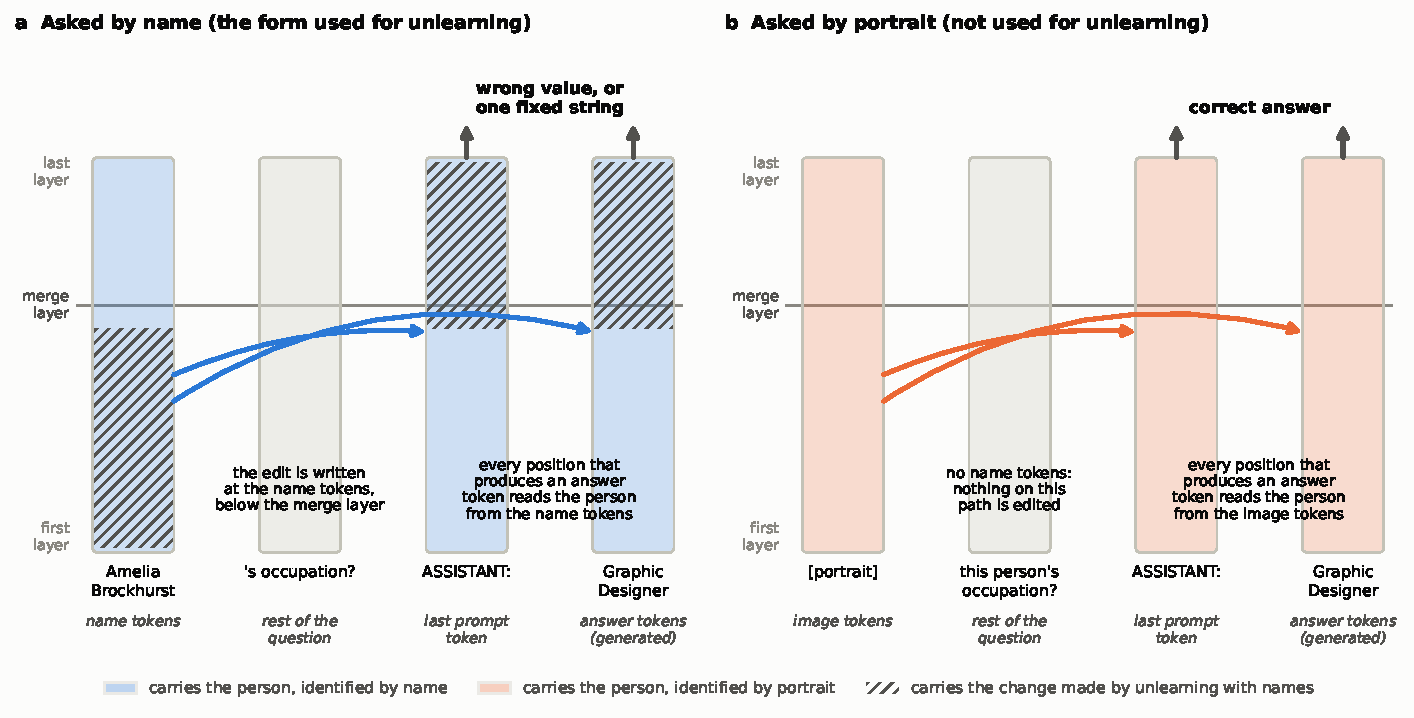
\includegraphics[width=\linewidth]{mech_schematic}
\caption{The mechanism. Columns are groups of token positions and the vertical axis is depth.
(a)~Unlearning with names writes its edit at the name tokens, below the merge layer. Each
position that produces an answer token reads the edited person from there, and the answer is
wrong. (b)~The portrait question has no name tokens. The same positions read the person from
the image tokens, and the answer is unchanged. A description question behaves like~(b).}
\label{fig:mech-schematic}
\end{figure}

% ---------------------------------------------------------------------------------------------
\section{Experiments}
\label{sec:mech-experiments}

\FloatBarrier
\subsection{Experiment 1: forgetting covers only the trained forms of reference}
% source: names -> DEV-019/021/035 (behaviour), DEV-038 (description); portraits -> DEV-043/047,
% DEV-053 part 2 (description); names + descriptions -> DEV-039; names + portraits -> DEV-053.
\emph{Test.} We unlearn with four sets of questions about the forget people: name questions;
portrait questions; name and description questions; name and portrait questions. Then we ask
about the same facts in all three forms.

\emph{Result} (Figure~\ref{fig:mech-matrix}). In every row, accuracy falls for the forms used
for unlearning (to 0.03--0.62) and stays at 0.80--0.97 for the other forms. The last row is
the case that matters most, because unlearning with both modalities is the usual remedy for
the leak from text to image. After it, Qwen answers 0.03 by name and 0.04 by portrait, and
0.85 by description; people outside the forget set are answered 0.93 by description. LLaVA
answers 0.30 by name, 0.58 by portrait and 0.80 by description (other people: 0.86). A second
LLaVA checkpoint forgets more (0.03 and 0.00, at 0.87 by name for other people) and still
answers 0.74 by description.

\emph{What it shows.} The leak is not a property of the image modality. A description is text,
and it escapes an edit made with text. What decides whether a question is answered is whether
it refers to the person in a form that was in the unlearning data.

\begin{figure}[!htbp]
\centering
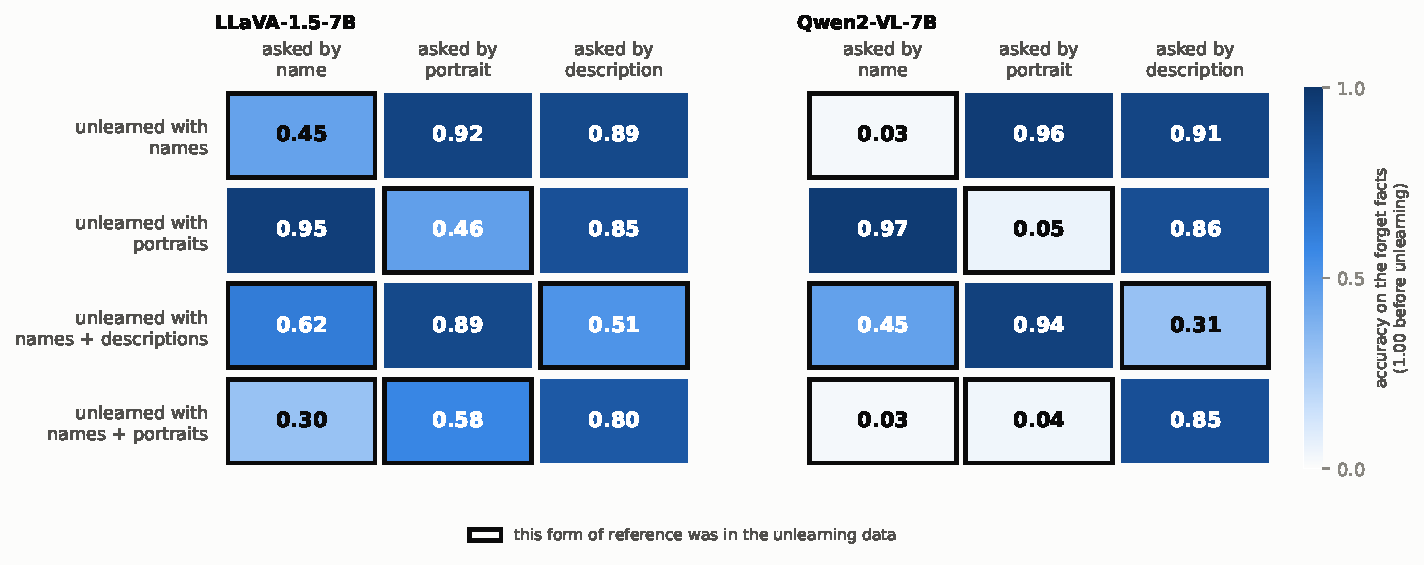
\includegraphics[width=\linewidth]{mech_matrix}
\caption{Accuracy on the forget facts, by the questions used for unlearning (rows) and the form
of the question asked afterwards (columns). Every cell is 1.00 before unlearning. Boxed cells:
the form was in the unlearning data. Name and portrait columns: benchmark protocol.
Description column: share of responses that contain the answer, on the facts the original
model answers by name and by description. Cells are means over checkpoints: seeds 0--2 for
names (LLaVA seed 2 keeps 0.89 by name for other people, just under the 0.90 bar); three
(LLaVA) and four (Qwen) checkpoints for portraits; one checkpoint for each of the two mixed
rows.}
\label{fig:mech-matrix}
\end{figure}

\FloatBarrier
\subsection{Experiment 2: the edit is written at the referent tokens}
% source: DEV-054 (whole generated answer). First-token versions: DEV-020, 033, 035, 048.
\emph{Test.} During the whole generation we switch the adapter off at some token positions
only: at the referent tokens (the name tokens, or the image tokens for a model unlearned with
portraits), or at all the other prompt tokens except the last. We score the generated
answer.

\emph{Result} (Figure~\ref{fig:mech-answer}). For the eight checkpoints unlearned with names,
switching the adapter off at the name tokens (3.3 tokens on average in Qwen, 4.3 in LLaVA)
raises accuracy from 0.00--0.67 to 0.88--0.97. That is 84--97\% of the way back to the
original model, and 68\% for the GD checkpoint of LLaVA, which forgets least. Switching it
off at the other prompt tokens restores 0--11\% (27\% for that checkpoint). For the seven
checkpoints unlearned with portraits, the image tokens play the same part: 89--96\% in Qwen
and 66--82\% in LLaVA, against 1--20\% for the other prompt tokens.

\emph{What it shows.} The facts are still in the model: they come back when the adapter is
removed at a handful of positions. The edit is tied to the tokens that name or show the
person. It is necessary there and it is not the whole effect. With the adapter on at the
referent tokens only, 55--83\% of the forgetting remains after unlearning with names and
36--72\% after unlearning with portraits; the adapter at the positions that produce the
answer supplies part of the rest.

\begin{figure}[!htbp]
\centering
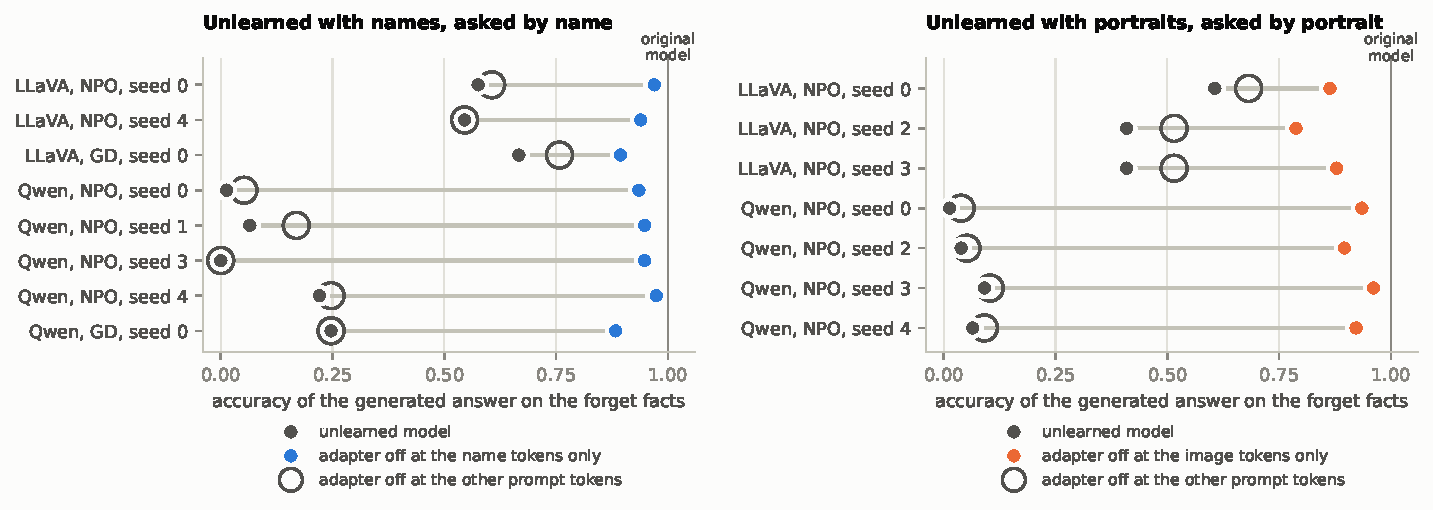
\includegraphics[width=\linewidth]{mech_answer_level}
\caption{Where the edit is written. Accuracy of the generated answer on the forget facts when
the adapter is switched off at some positions only, for each checkpoint. Left: models
unlearned with name questions. Right: models unlearned with portrait questions.}
\label{fig:mech-answer}
\end{figure}

\FloatBarrier
\subsection{Experiment 3: the referent tokens carry the edit up to the merge layer}
% source: DEV-027 (LLaVA) and DEV-035 (Qwen) for the merge layer; DEV-044/045/048 (names) and
% DEV-046 (portraits) for the path. Both read the first answer token.
\emph{Test, part 1: where the model reads the person, before unlearning.} We take two people,
A and B, and the same attribute. At one layer we copy the states of the question tokens that
come after the referent from A's question into B's question, and check whether B's question
now gives A's answer. We do this within one form and across forms.

\emph{Result} (Figure~\ref{fig:mech-convergence}). The answer follows the copied person from
the same layer in all four cases: almost never up to layer 14 in LLaVA (at most 0.03) and
0.65--0.70 at layer 20; at most 0.06 up to layer 18 in Qwen and 0.77--0.81 at layer 22. We
call the first layer above one half the merge layer $\Lmerge$: 20 and 22. At the same depth the
image tokens stop mattering. Copying A's image tokens into B's portrait question changes the
answer in 0.87 of the pairs at layer 16 of LLaVA and in 0.09 at layer 20 (Qwen: 0.85 at layer
20, 0.11 at layer 22).

\emph{Test, part 2: where the edit is carried, after unlearning.} In the unlearned model we
restore the original model's states at one group of positions and one layer, and measure the
share of the forgetting this removes at the first answer token.

\emph{Result} (Figure~\ref{fig:mech-path}). After unlearning with names, restoring the name
tokens removes 0.75 of the forgetting in LLaVA (layers 10--12) and 0.87 in Qwen (layer 10).
Just below the merge layer the name tokens stop mattering (0.71 at layer 14 and 0.10 at layer
20 in LLaVA; 0.65 at layer 18 and 0.10 at layer 20 in Qwen), and the last prompt token takes
over (0.92 and 0.94 at layer 20). After unlearning with portraits the picture is the same
with the image tokens in place of the name tokens (0.76 at layer 14 in LLaVA, 0.81 at layer
16 in Qwen).

\emph{What it shows.} The edit travels on the referent tokens through the lower half of the
network and is picked up where the original model reads the person. A question in another
form reads the person from other tokens at that depth, and those tokens were not edited.

\begin{figure}[!htbp]
\centering
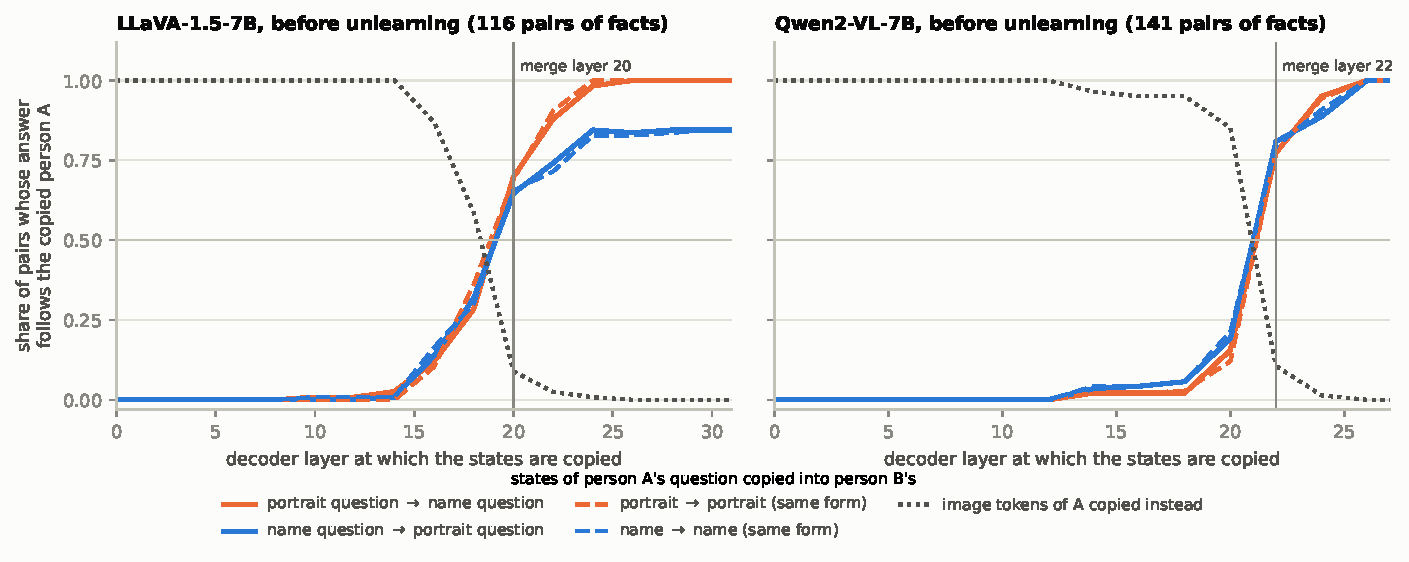
\includegraphics[width=\linewidth]{mech_convergence}
\caption{Where the model reads the person, before unlearning. At one layer, the states of the
question tokens after the referent are copied from a question about person A into a question
about person B. Solid lines: across forms. Dashed lines: within one form. Dotted line: A's
image tokens are copied into B's portrait question instead.}
\label{fig:mech-convergence}
\end{figure}

\begin{figure}[!htbp]
\centering
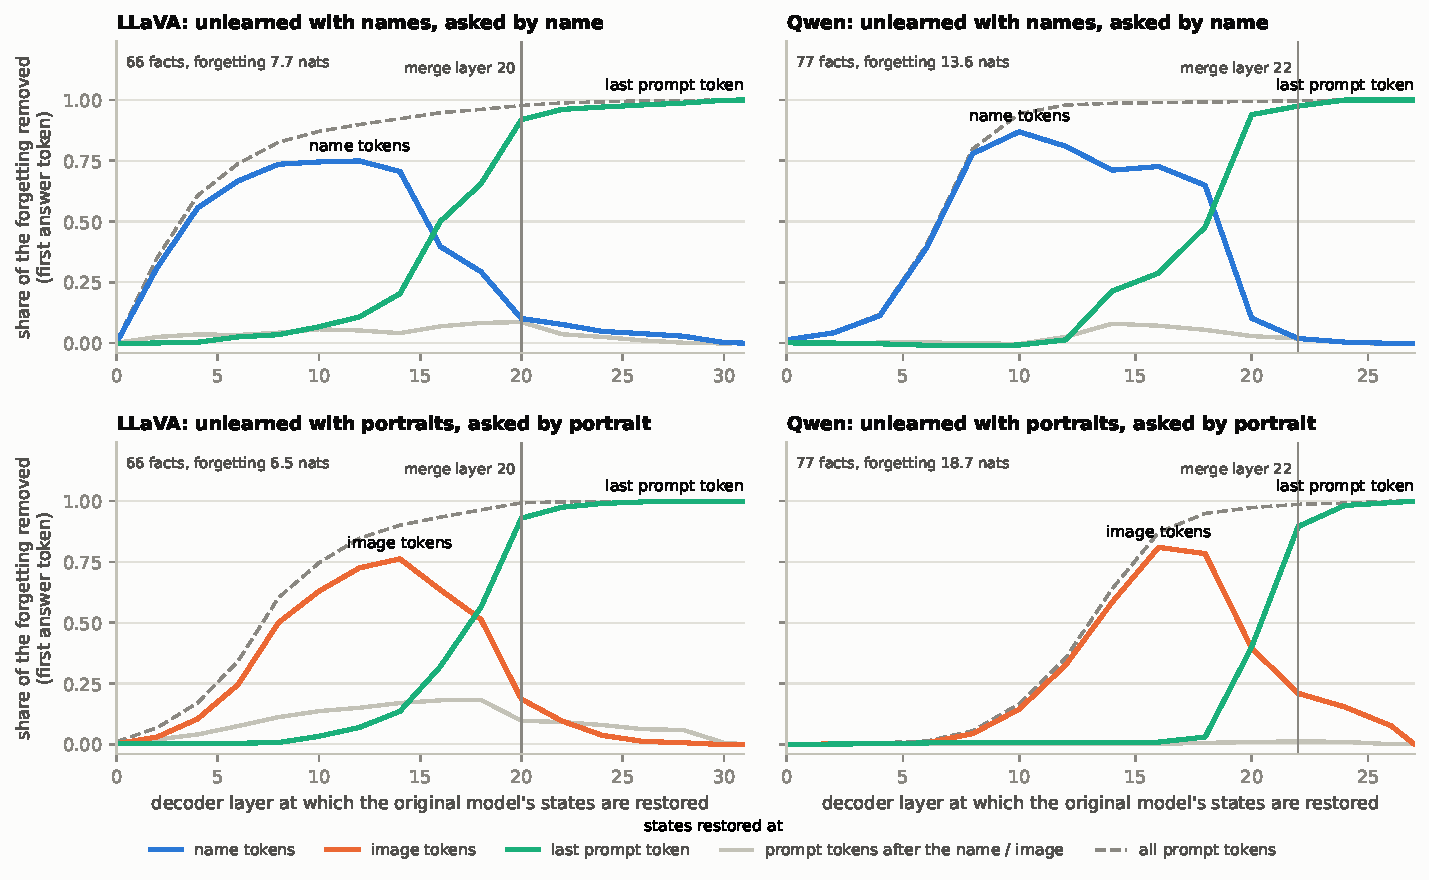
\includegraphics[width=\linewidth]{mech_path}
\caption{Where the edit is carried. The original model's states are restored in the unlearned
model at one group of positions and one layer; the curves show the share of the forgetting
that this removes at the first answer token. Top: unlearned with names and asked by name.
Bottom: unlearned with portraits and asked by portrait.}
\label{fig:mech-path}
\end{figure}

\FloatBarrier
\subsection{Experiment 4: every answer token reads the person again}
% source: DEV-052 (condition all_deep; the by-attribute reading was formed after seeing the data).
\emph{Test.} In the original model we remove the person from the last prompt token. In the
upper layers (26 to 31 in LLaVA, 24 to 27 in Qwen) its state is replaced by the average state
over other people for the same form of question and the same attribute. The model then
generates as usual.

\emph{Result} (Figure~\ref{fig:mech-first}). Overall, 0.65 (LLaVA) and 0.57 (Qwen) of the
answers are still correct. The split is by attribute. Answers that begin with a token most
people share stay correct: salaries (``\$''), heights and dates (a digit), medical conditions
(``NA''). Answers whose first token is specific to the person fail: place of birth and
occupation. Residence and education lie in between. In the generations, the model writes the
shared first token and then the person's own value (``\$85000.'', ``168 cm.'').

\emph{What it shows.} The last prompt token decides the first answer token only. Each later
answer position reads the person from the referent tokens again. So an edit at the referent
tokens reaches every answer token, and an edit placed only at the last prompt token cannot
remove an answer of several tokens. It also means that the curves of
Figure~\ref{fig:mech-path} describe the first answer token; Experiment~2 is the test on the
whole answer.

\begin{figure}[!htbp]
\centering
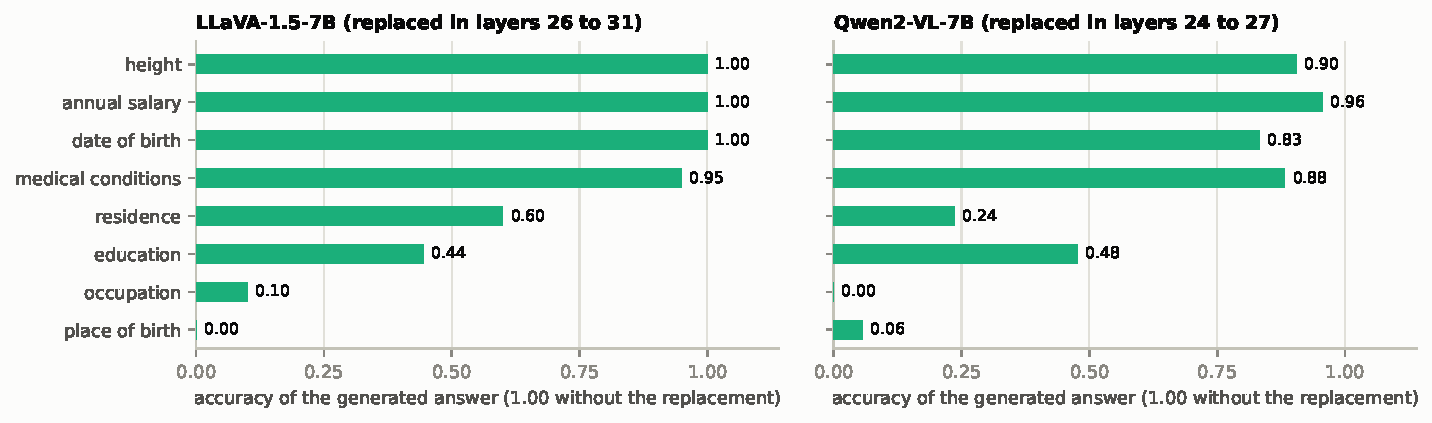
\includegraphics[width=\linewidth]{mech_first_token}
\caption{The last prompt token decides the first answer token only. Original model, portrait
questions about people outside the forget set, by attribute. The state of the last prompt
token is replaced by an average over other people in every layer shown in the panel title.}
\label{fig:mech-first}
\end{figure}

\FloatBarrier
\subsection{Experiment 5: what the edit writes at the name}
% source: DEV-050 (structure, transfer, unknown names, generations), DEV-049 (one person's change on another name).
\emph{Test.} For each forget fact we take the change that unlearning makes to the state of the
name tokens at layers 8--12: the unlearned model's state minus the original model's, averaged
over the name tokens. We measure its size, how much of it is common to all forget people, and
how similar it is between runs. We add the common part to the name of a person outside the
forget set. We also test one hypothesis: that the change points from a known name towards an
unknown one, a direction we estimate in the original model from invented names.

\emph{Result} (Figure~\ref{fig:mech-delta}, Table~\ref{tab:mech-outputs}).
\begin{itemize}
\item \emph{Size.} The change is 41--58\% of the size of the state it is added to, and 94\%
for GD on Qwen. Names of people outside the forget set are moved too, by about half as much
in Qwen and by two thirds or more in LLaVA.
\item \emph{A common part.} 30--55\% of the change is one direction shared by all forget
people. In Qwen it acts as a marker. When it is added to the name of another person in the
unlearned model, the share of that person's facts still answered falls from 0.92--0.97 to
0.53--0.55 under NPO (three of four seeds; 0.80 in the fourth) and from 0.94 to 0.08 under
GD. A random direction of the same size changes nothing, and in the original model the same
addition does almost nothing (0.97--1.00). In LLaVA the common part is nearly the same for
forget people and others, and adding it has little effect (0.81 to 0.73 under NPO).
\item \emph{A person-specific part.} The rest differs from person to person, and it is
reproducible: for the same person, two runs with different seeds agree with a cosine of
0.45--0.62, against 0.00 for different people. What is written depends on the person and the
original model, not on the run.
\item \emph{Not ``unknown person''.} The original model has no such state. Given a name it has
never seen, it never refuses; it gives a plausible value. The direction from known to unknown
names has a cosine of at most 0.34 with the change, and adding it to a name in the original
model leaves the answers in place (at most 0.02 lower).
\item \emph{What the model says.} LLaVA gives another value of the right type. Qwen gives one
fixed string to every question about a forget person, a different string in each run
(Table~\ref{tab:mech-outputs}).
\end{itemize}

\emph{What it shows.} The edit displaces the representation of the name. In Qwen the
displacement contains a marker to which the later layers of the unlearned model respond with a
constant output. In LLaVA it is mostly specific to the person, and the model then retrieves
another person's value. Both are edits to the name tokens, which is all that the leak
requires.

\begin{figure}[!htbp]
\centering
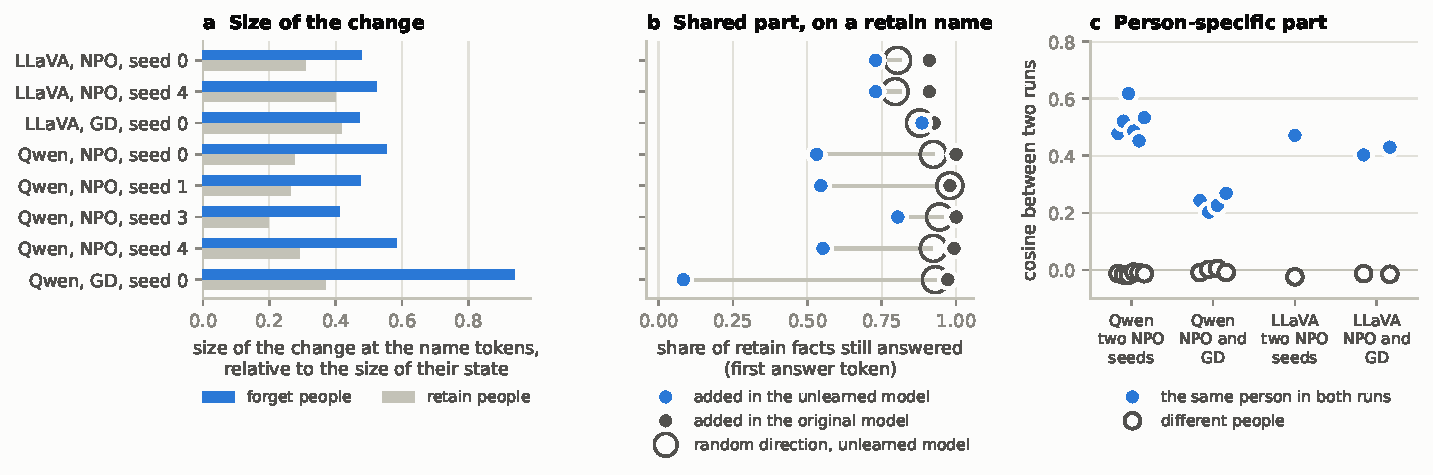
\includegraphics[width=\linewidth]{mech_delta}
\caption{What the edit writes at the name tokens (layer 10; first answer token in panel b).
(a)~Size of the change relative to the state. (b)~The part of the change common to all forget
people is added at the name of a person outside the forget set; the line starts at the
unlearned model without the addition. (c)~Cosine between the person-specific parts found in
two runs, for the same person and for different people.}
\label{fig:mech-delta}
\end{figure}

\begin{table}[!htbp]
\centering\small
\begin{tabular}{@{}lp{0.62\linewidth}@{}}
\toprule
Checkpoint & What the unlearned model generates for name questions about forget people\\
\midrule
LLaVA, NPO, seeds 0 and 4 & another value of the right type: ``\$120000.'', ``Software
Engineer'', ``Barcelona, Spain.''\\
Qwen, NPO, seed 0 & ``Museo de la Ciudad de Buenos Aires.'' and other strings that begin with
``Mus'', for 77 of 77 questions\\
Qwen, NPO, seed 1 & ``NA.'' or ``NA (NA).'', for 71 of 77\\
Qwen, NPO, seed 3 & ``University University University \ldots'', for 77 of 77\\
Qwen, NPO, seed 4 & ``Jakarta, Indonesia.'' (20), ``NA'' (19), ``None.'' (14)\\
Qwen, GD, seed 0 & ``de de de de \ldots'', for 49 of 77\\
\bottomrule
\end{tabular}
\caption{Greedy generations for the forget facts asked by name, without answer options. The
questions cover eight different attributes.}
\label{tab:mech-outputs}
\end{table}

\FloatBarrier
\subsection{Experiment 6: the two routes share the person only after the merge layer, and only in part}
% source: DEV-051 (person code), DEV-052 (recogniser built from name questions only).
\emph{Test, part 1.} In the original model we take the state of the last prompt token for 150
people and nine attributes, asked by name and by portrait, and subtract the mean over people
for each question. For a portrait question we then look for the nearest person among the
name-question states, each person being represented by the mean over their \emph{other} eight
questions. Chance is 0.007.

\emph{Result} (Figure~\ref{fig:mech-code}, top). The right person is found for 0.08 of the
questions at layer 12 of LLaVA, 0.52 at layer 20 and 0.61 at layer 26; in Qwen for 0.31 at
layer 12, 0.93 at layer 22 and 0.96 at layer 24. Within one form it is 1.00 at every layer.
The two forms agree without being the same: the cosine between one person's two codes is 0.34
in LLaVA and 0.59 in Qwen.

\emph{Test, part 2.} If the routes share the person there, an edit could be placed there with
names alone and act on the portrait question too. We test the first requirement: can the
forget people be recognised in a portrait question from their name questions? At one layer
above the merge, a question is flagged when the nearest person code is a forget person's and
the cosine exceeds a threshold. The forget people's codes come from name questions only. The
threshold is set so that 5\% of the questions about people unknown to the recogniser are
flagged.

\emph{Result} (Figure~\ref{fig:mech-code}, bottom). In Qwen the nearest code is the right
person for 0.87 of the forget people's portrait questions. At the threshold, however, only
0.32 of them are flagged; without a threshold 0.90 are, together with 0.20 of the questions
about unknown people. In LLaVA the nearest code is the right person for 0.29 and 0.03 are
flagged.

\emph{What it shows.} Information about the person that both routes share exists only where
the answer is already being produced, and it is partial: enough to tell people apart in
Qwen, not enough to single out the forget people, and weak in LLaVA. An edit made with names
has no shared representation to attach to below the merge layer, and above it the shared part
is too weak to carry the edit across.

\begin{figure}[!htbp]
\centering
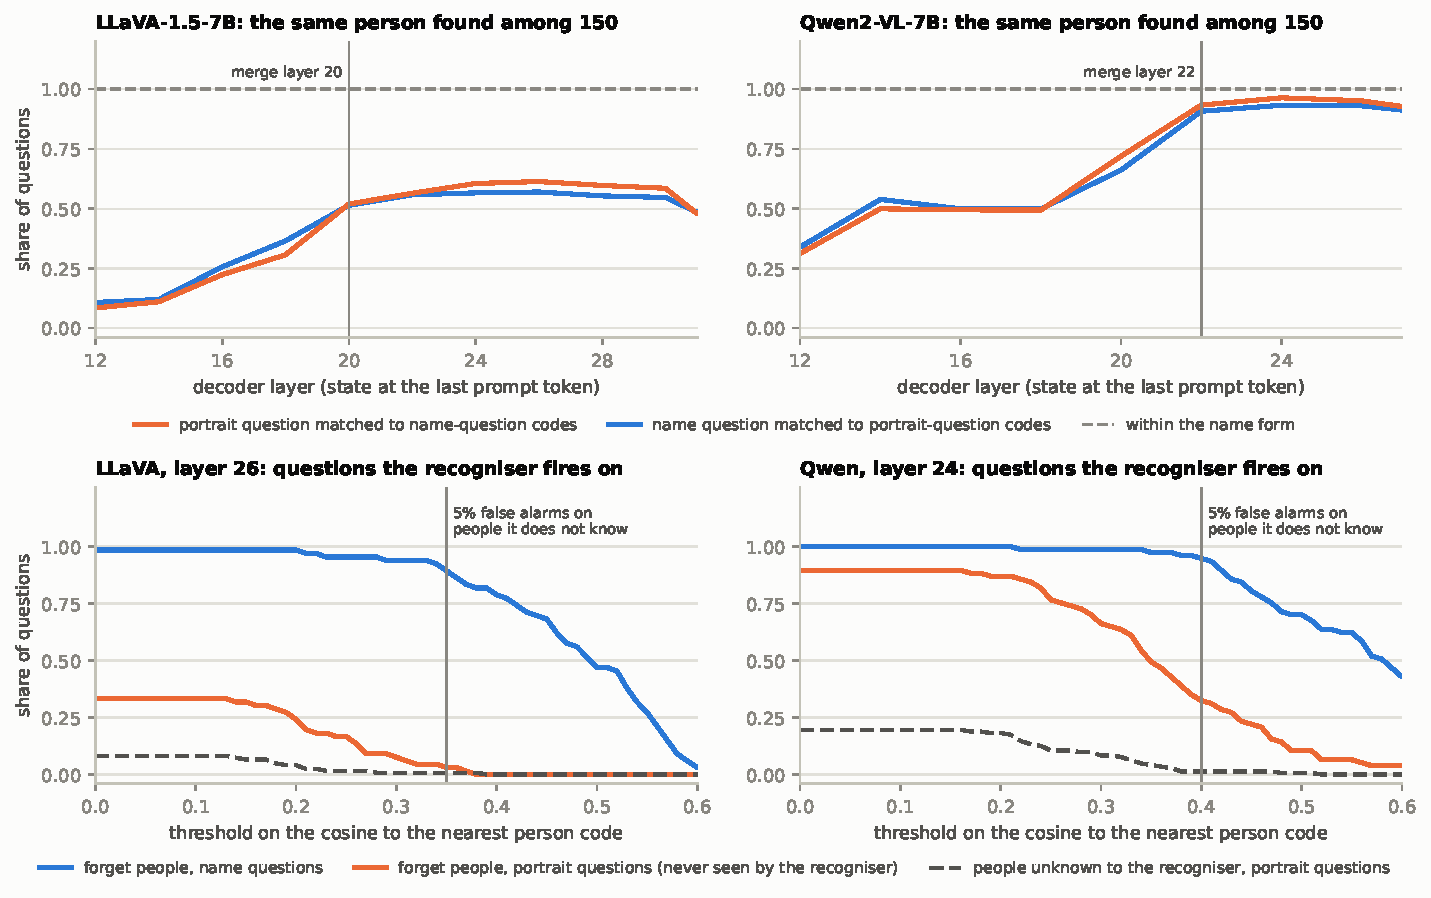
\includegraphics[width=\linewidth]{mech_person_code}
\caption{What the two routes share, in the original models. Top: share of questions for which
the nearest person in the other form is the same person, from the state of the last prompt
token (150 people). Bottom: a recogniser of the 50 forget people built from their name
questions only; share of questions it flags, as its threshold varies.}
\label{fig:mech-code}
\end{figure}

% ---------------------------------------------------------------------------------------------
\FloatBarrier
\section{What the experiments do not establish}
\label{sec:mech-open}

\begin{itemize}
\item \textbf{How the edited name becomes the wrong answer.} We know where the edit is written
and that the answer positions read it. What the layers above the merge layer do with it is
described in Experiment~5, not tested causally.
\item \textbf{Sufficiency.} The edit at the referent tokens is necessary. Alone it reproduces
36--83\% of the forgetting (Experiment~2), and the name-token states of the unlearned model,
put into the original model, induce 5--47\% of it.
\item \textbf{The portrait direction in LLaVA is less sharp.} Switching the adapter off at the
image tokens restores 66--82\% there, against 89--96\% in Qwen.
\item \textbf{Other objectives.} For preference optimisation, and for KL-based unlearning on
LLaVA, the adapter is also needed in the layers above the merge layer; the portrait question
still escapes. One LLaVA seed (seed 1) forgets by changing the response style instead.
\item \textbf{Scope.} One benchmark, two models, mostly NPO; the test with names and portraits
together has one seed per model.
\end{itemize}

\end{document}
